\input{"../../../preamble"}

\begin{document}

\title{CSC263-Notes-03-02-2015}

\input{"../csc263-header"}
\rhead{March 2, 2015}

\section*{Lecture 15}

\reversemarginpar
\mpreadings

\noindent Sections 22.1, 22.2 \\

\mpselftest

\noindent Exercises 22.1-1, 22.1-2, 22.2-1

\subsection*{Graphs}

\noindent A graph $G=(V,E)$ consists of a set of ``vertices'' (or ``nodes'') $V$ and
a set of ``edges'' (or ``arcs'') $E$. \\

\noindent In a \textbf{directed} graph, each edge is a pair of two vertices $(u,v)$ is considered
different from the pair $(v,u)$, self-loops of the form $(u,u)$ are allowed. \\

\noindent In an \textbf{undirected} graph each set of two vertices $\{u,v\}$ (so $\{u,v\}$ and
$\{v,u\}$ are the same) and self loops are disallowed. \\

\noindent A \textbf{weighted} graph is either directed or undirected. Each edge $e \in E$ is assigned
a real number $w(e)$ called its weight. \\

\noindent \textit{A story to solve with a graph:} \\
There is a party. 4 couples attend the party. Hand shaking occurs at the party.
Hand shaking is reciprocal. Nobody shakes hands with their date. No duplicate answers
when a person $P$ asks everyone else how many hands did they shake. How many hands did $P$ shake? \\

\begin{tabular}{c c c}
	directed & undirected & weighted \\
	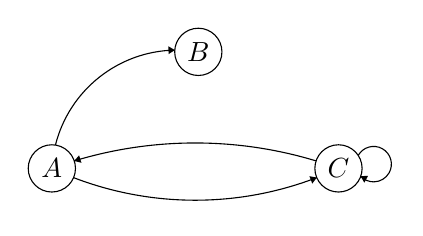
\begin{tikzpicture}[scale=0.1]
	\tikzstyle{every node}+=[inner sep=0pt]
	\draw [black] (16.7,-33.5) circle (3);
	\draw (16.7,-33.5) node {$A$};
	\draw [black] (35.3,-18.7) circle (3);
	\draw (35.3,-18.7) node {$B$};
	\draw [black] (53.1,-33.5) circle (3);
	\draw (53.1,-33.5) node {$C$};
	\draw [black] (17.154,-30.539) arc (165.88777:91.13069:15.955);
	\fill [black] (32.31,-18.48) -- (31.5,-17.99) -- (31.52,-18.99);
	\draw [black] (19.544,-32.548) arc (106.88074:73.11926:52.881);
	\fill [black] (19.54,-32.55) -- (20.46,-32.79) -- (20.16,-31.84);
	\draw [black] (50.34,-34.674) arc (-68.96339:-111.03661:43.012);
	\fill [black] (50.34,-34.67) -- (49.41,-34.49) -- (49.77,-35.43);
	\draw [black] (55.601,-31.865) arc (150.91297:-137.08703:2.25);
	\fill [black] (55.92,-34.49) -- (56.38,-35.32) -- (56.86,-34.44);
	\end{tikzpicture} &
	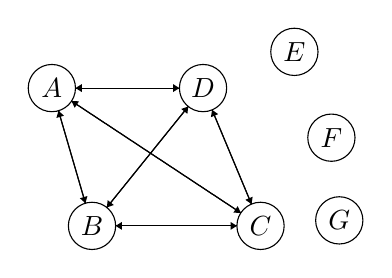
\begin{tikzpicture}[scale=0.1]
	\tikzstyle{every node}+=[inner sep=0pt]
	\draw [black] (19.8,-21.5) circle (3);
	\draw (19.8,-21.5) node {$A$};
	\draw [black] (24.9,-39) circle (3);
	\draw (24.9,-39) node {$B$};
	\draw [black] (46.3,-39) circle (3);
	\draw (46.3,-39) node {$C$};
	\draw [black] (39,-21.5) circle (3);
	\draw (39,-21.5) node {$D$};
	\draw [black] (50.6,-16.9) circle (3);
	\draw (50.6,-16.9) node {$E$};
	\draw [black] (55.3,-27.8) circle (3);
	\draw (55.3,-27.8) node {$F$};
	\draw [black] (56.3,-38.3) circle (3);
	\draw (56.3,-38.3) node {$G$};
	\draw [black] (20.64,-24.38) -- (24.06,-36.12);
	\fill [black] (24.06,-36.12) -- (24.32,-35.21) -- (23.36,-35.49);
	\draw [black] (24.06,-36.12) -- (20.64,-24.38);
	\fill [black] (20.64,-24.38) -- (20.38,-25.29) -- (21.34,-25.01);
	\draw [black] (27.9,-39) -- (43.3,-39);
	\fill [black] (43.3,-39) -- (42.5,-38.5) -- (42.5,-39.5);
	\draw [black] (43.3,-39) -- (27.9,-39);
	\fill [black] (27.9,-39) -- (28.7,-39.5) -- (28.7,-38.5);
	\draw [black] (22.3,-23.15) -- (43.8,-37.35);
	\fill [black] (43.8,-37.35) -- (43.4,-36.49) -- (42.85,-37.32);
	\draw [black] (43.8,-37.35) -- (22.3,-23.15);
	\fill [black] (22.3,-23.15) -- (22.7,-24.01) -- (23.25,-23.18);
	\draw [black] (26.78,-36.66) -- (37.12,-23.84);
	\fill [black] (37.12,-23.84) -- (36.23,-24.15) -- (37.01,-24.77);
	\draw [black] (37.12,-23.84) -- (26.78,-36.66);
	\fill [black] (26.78,-36.66) -- (27.67,-36.35) -- (26.89,-35.73);
	\draw [black] (40.15,-24.27) -- (45.15,-36.23);
	\fill [black] (45.15,-36.23) -- (45.3,-35.3) -- (44.38,-35.69);
	\draw [black] (45.15,-36.23) -- (40.15,-24.27);
	\fill [black] (40.15,-24.27) -- (40,-25.2) -- (40.92,-24.81);
	\draw [black] (36,-21.5) -- (22.8,-21.5);
	\fill [black] (22.8,-21.5) -- (23.6,-22) -- (23.6,-21);
	\draw [black] (22.8,-21.5) -- (36,-21.5);
	\fill [black] (36,-21.5) -- (35.2,-21) -- (35.2,-22);
	\end{tikzpicture} &
	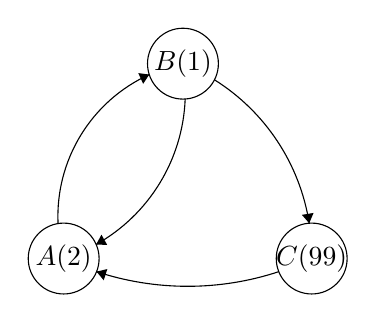
\begin{tikzpicture}[scale=0.15]
	\tikzstyle{every node}+=[inner sep=0pt]
	\draw [black] (22.7,-37.9) circle (3);
	\draw (22.7,-37.9) node {$A(2)$};
	\draw [black] (32.8,-21.4) circle (3);
	\draw (32.8,-21.4) node {$B(1)$};
	\draw [black] (43.7,-37.9) circle (3);
	\draw (43.7,-37.9) node {$C(99)$};
	\draw [black] (22.225,-34.944) arc (-177.38248:-245.56088:13.203);
	\fill [black] (29.95,-22.32) -- (29.02,-22.2) -- (29.43,-23.11);
	\draw [black] (32.988,-24.389) arc (-2.21508:-60.72829:14.777);
	\fill [black] (25.45,-36.71) -- (26.39,-36.75) -- (25.9,-35.88);
	\draw [black] (35.467,-22.766) arc (57.96697:8.93102:17.537);
	\fill [black] (43.49,-34.91) -- (43.86,-34.04) -- (42.87,-34.2);
	\draw [black] (40.915,-39.011) arc (-71.73132:-108.26868:24.613);
	\fill [black] (25.48,-39.01) -- (26.09,-39.74) -- (26.4,-38.79);
	\end{tikzpicture}

\end{tabular} \\

\subsubsection*{Standard operations on graphs}

\begin{itemize}
	\item add a vertex; remove a vertex; add an edge; remove and edge
	\item edge query
		\begin{itemize}
			\item given two vertices $u,v$ find out if a directed edge $(u,v)$ or
				undirected edge $\{u,v\}$ is in the graph
		\end{itemize}
	\item neighbourhood
		\begin{itemize}
			\item given a vertex $u$ in an undirected graph, find the set of vertices $v$
				such that $\{u,v\}$ is an edge
		\end{itemize}
	\item in-neighbourhood, out-neighbourhood
		\begin{itemize}
			\item apply to directed graph
			\item in-neighbourhood $\rightarrow$ given a vertex $u$ in a directed graph, set of
				vertices $v$ such that $(v,u) \in G$
			\item out-neighbourhood $\rightarrow$ given a vertex $u$ in a directed graph, set of
				vertices $v$ such that $(u,v) \in G$
		\end{itemize}
	\item degree, in-degree, out-degree
		\begin{itemize}
			\item degree $\rightarrow$ size of neighbourhood
		\end{itemize}
	\item traversal
		\begin{itemize}
			\item visit each vertex of the graph to perform some task
		\end{itemize}
\end{itemize}

\subsubsection*{Definitions}

\noindent \textbf{path}:= a set of edges to get from one vertex to another: $(v,u_1),(u_1,u_2),\ldots,(u_{k-1},w)$ \\
\textbf{length of path}:= number of edges\\
\textbf{simple path}:= no repeated edge or vertex \\
\textbf{cycle}:= a path with the end vertex equal to start vertex\\
\textbf{simple cycle}:= a cycle with no repeated edge or vertex \\
\textbf{tree}:= undirected graph that is acylic and connected \\
\textbf{forest}:= acyclic graph (collection of disjoint trees, each one a ``connected component'')\\

\subsubsection*{Adjacency Matrix}

\noindent Let $V = {v_1,v_2,\ldots,v_n}$. Store edges in $[n \cdot n]$ array: \\

\begin{tabular}{l | l l l l l l l}
	& A & B & C & D & E & F & G \\ \hline
  A & 0 & 1 & 1 & 1 & 0 & 0 & 0 \\
  B & 1 & 0 & 1 & 1 & 0 & 0 & 0 \\
  C & 1 & 1 & 0 & 1 & 0 & 1 & 0 \\
  D & 1 & 1 & 1 & 0 & 1 & 0 & 1 \\
  E & 0 & 0 & 0 & 0 & 0 & 0 & 0 \\
  F & 0 & 0 & 1 & 1 & 0 & 0 & 0 \\
  G & 0 & 0 & 0 & 1 & 0 & 0 & 0 \\
\end{tabular} \\

\noindent Undirected graphs: matrix is symmetric ($A[i,j] = A[j.i]$) \\
Space $\in Theta(n^2)$, edge queries take time $\Theta(1)$. \\
Weighted graph: store $w(v_i,v_j)$ in $A[i,j]$ if $(v_i,v_j)$ in $E$; special value (-1/0/$\infty$) otherwise (depending on application)

\subsubsection*{Adjacency List}

Let V = ${v_1,v_2,\ldots,v_n}$. Store edges in a list of lists: ``main'' list has positions $1,\ldots,n$ (one for each vertex); \\
sub-list[$i$] contains $j_1,\ldots,j_{k_i}$ such that $(v_i,v_{j_1}), \ldots, (v_i,v_{i_{k_i}})$ are all edges from $v_i$. \\
Undirected graph: edge $\{u,v\}$ stored twice ($u$ in sub-list[$v$] and $v$ in
sub-list[$u$]). \\

\begin{tabular}{l | l}
	A & b,c \\
	B & \\
	C & a,b,c \\
	D & e \\
	E & \\
\end{tabular} \\

\noindent Space $\in \Theta(n+m)$ (where $n = |V|$ and $m = |E|$). \\
Edge queries in time $\Theta(\log n)$ (actually, $\Theta(\log (\textrm{max degree} )))$ if sub-lists stored in balanced trees.



\end{document}
